%! Author = leocr
%! Date = 04/01/2025

% Preamble
\documentclass[12pt]{article}

% Packages
\usepackage[top=1in, bottom=1.2in, left=1in, right=1in]{geometry}
\usepackage{amsmath}
\usepackage{upgreek}
\usepackage{graphicx}
\usepackage{wrapfig}
\usepackage{hyperref}
\usepackage{tikzexternal}
\setlength{\parindent}{0pt}




% Document
\begin{document}
    \section{Introduction}
    The aim of this work is to estimate the parameters of the SIR model.
    In particular, I will focus on the first wave of contagion of the Coronavirus pandemic in Italy.

    \begin{figure}[h!]
        \label{fig:covid_italy}
        \centering
        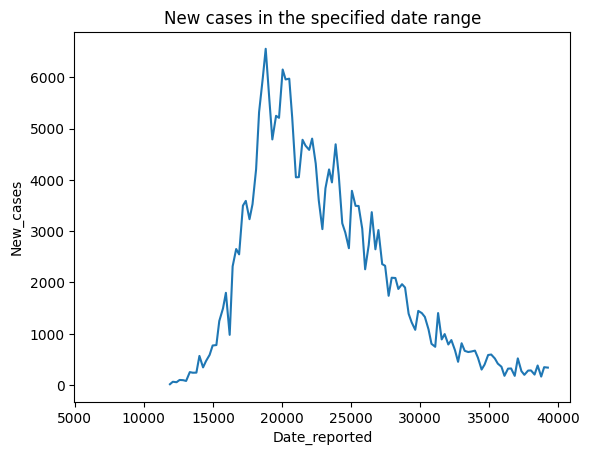
\includegraphics[width=.8\linewidth]{plots/real_data}
        \caption{New infections per day in Italy}
    \end{figure}

\pagebreak

    \section{Model \& Estimation}
    The model is as follows:
    \begin{equation}
        N_{t} = \gamma_1 N_{t-1} + \gamma_2 N_{t-1}  \ln N_{t-1} + U_t,
        \label{eq:model_eq}
    \end{equation}

    where $N_t$ is the total infected population at time $t$, and $U_t$ is the error term.

    \iffalse
    \begin{figure}[h!]
    \begin{center}
        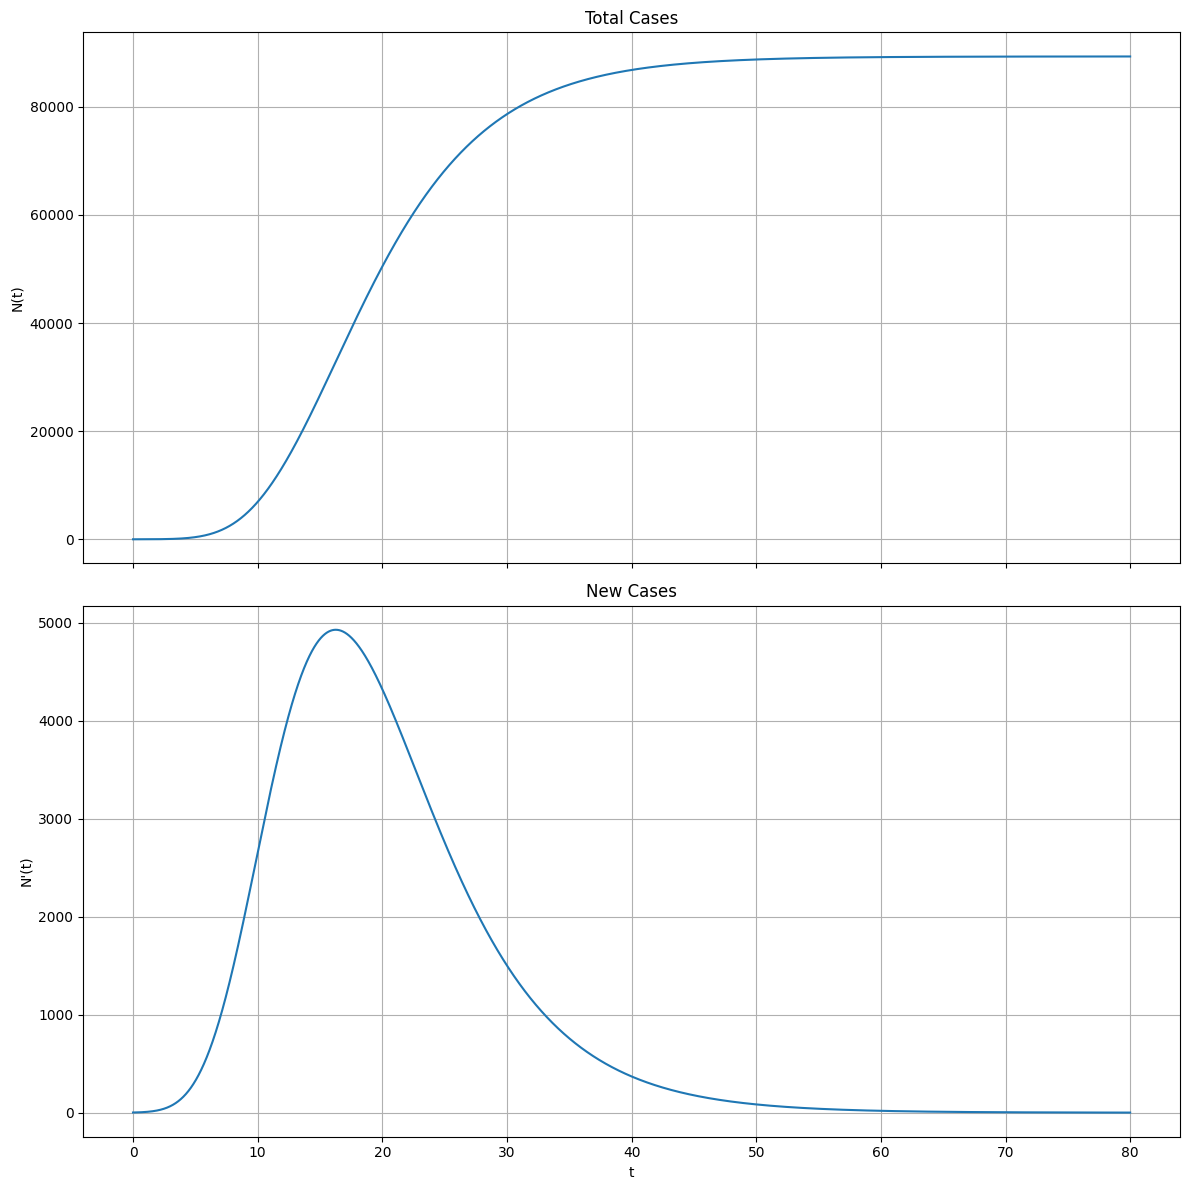
\includegraphics[width=\linewidth]{plots/num_int}
        \caption{The result of the numerical integration correctly reproduces the right-skewness of the contagion curve}
        \label{fig:num_int}
    \end{center}
    \end{figure}
    \fi

    The model has been estimated through GMM, using different combinations of the following instruments:
    \begin{itemize}
        \item $N_{t-1}$
        \item $N_{t-1}  \ln N_{t-1}$
        \item Daily average temperature in Italy $W_1$
        \item Daily average mobility in Italy, in particular the percent change from baseline of occupation of:
        \begin{itemize}
            \item Retail and recreation facilities $W_2$
            \item Transit stations $W_3$
        \end{itemize}
    \end{itemize}

    In particular:
    \begin{table}[h!]
        \centering
        \begin{tabular}{l|c}
            Model & Instruments \\ \hline
            1 & $N_{t-1}$ \, $W_1$ \\
            2 & $N_{t-1}$ \, $W_1$ \\
            3 & $N_{t-1}$ \, $N_{t-1}  \ln N_{t-1}$ \, $W_1$\, $W_2$\, $W_3$ \\
            4 & $W_1$\, $W_2$\, $W_3$  \\
        \end{tabular}
    \end{table}

    The results are as follows:
    \begin{table}[h!]
        \centering
        {
\newcommand{\sym}[1]{\ifmmode^{#1}\else\(^{#1}\)\fi}
\begin{tabular}{l*{4}{c}}
\hline\hline
                    &\multicolumn{1}{c}{Model 1}&\multicolumn{1}{c}{Model 2}&\multicolumn{1}{c}{Model 3}&\multicolumn{1}{c}{Model 4}\\
\hline
$\gamma_1$            &       1.735\sym{***}&       1.722\sym{***}&       1.717\sym{***}&       1.726\sym{***}\\
                    &    (0.0217)         &    (0.0205)         &    (0.0201)         &    (0.0203)         \\
\hline
$\gamma_2$            &     -0.0593\sym{***}&     -0.0583\sym{***}&     -0.0579\sym{***}&     -0.0586\sym{***}\\
                    &   (0.00177)         &   (0.00167)         &   (0.00163)         &   (0.00165)         \\
\hline
Observations        &         129         &         129         &         129         &         129         \\
J-stat              &       8.520         &       11.60         &       13.08         &       2.175         \\
DoF                 &           1         &           1         &           4         &           2         \\
\hline\hline
\end{tabular}
}

        \caption{GMM results: standard errors are in parentheses and \sym{*}\(p<0.10\), \sym{**}\(p<0.05\), \sym{***}\(p<0.01\)}
    \end{table}

    From Hansen J-test of model 4 and EHS test of model 3 and 4 we can see that $N_{t-1}$ is endogenous with respect to $U_t$, and thus only model 4 is well-defined.

    \begin{figure}[h!]
        \centering
        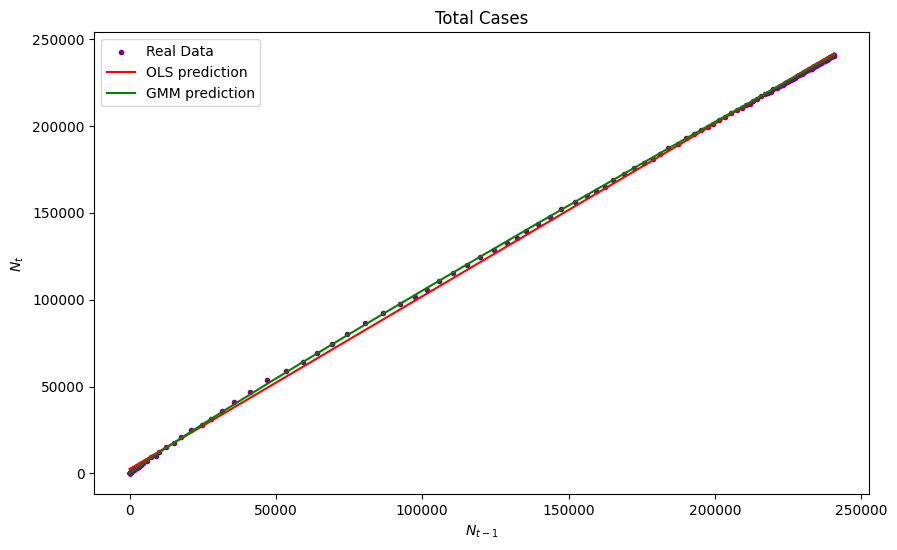
\includegraphics[width=0.6\linewidth]{plots/regression_comparison_1}\quad
        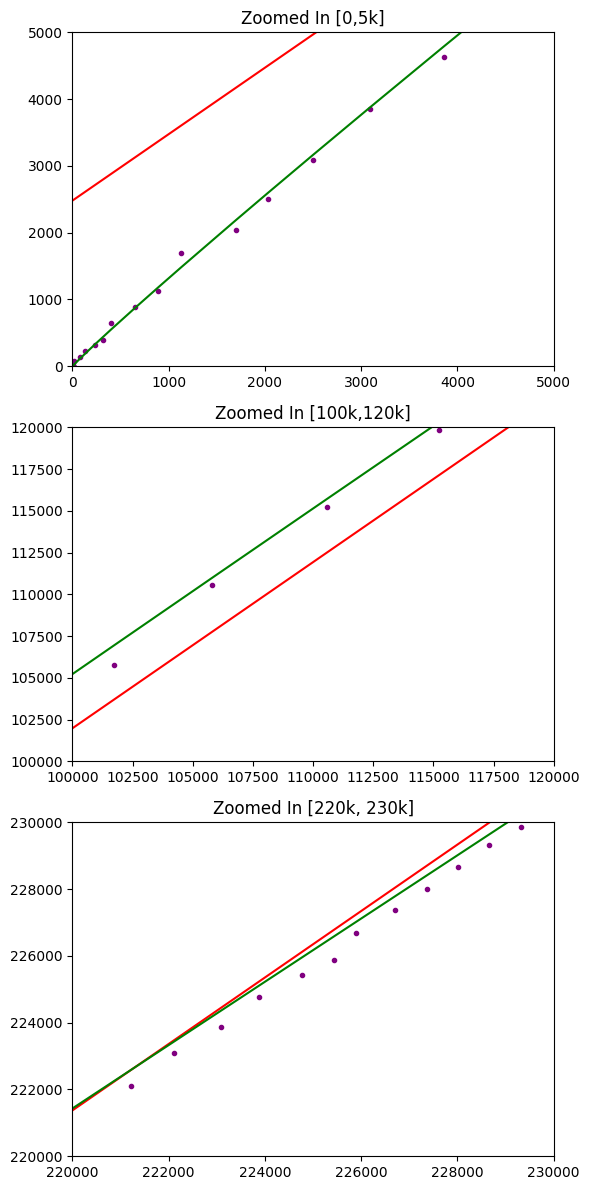
\includegraphics[width=0.2\linewidth]{plots/regression_comparison_2}
        \caption{$N_t$ vs $N_{t-1}$ comparison between OLS and Model 4}
        \label{fig:plot_gmm_ols_comp}
    \end{figure}

    \section{Explicit Solution}
    In continuous time, the model equation~\eqref{eq:model_eq} admits the following close form solution (i.e.\ total cases):
    \begin{equation}
        N(t)=\exp\Biggl(\frac{K e^{\gamma_2t}-\gamma_1+1}{\gamma_2}\Biggr), \qquad K=\gamma_1+\gamma_2\ln N_0,
    \end{equation}
    And derivative (i.e.\ new cases):
    \begin{equation}
        \dot N(t) =K\,e^{\gamma_2t}\,N(t).
    \end{equation}

    $K$ can therefore be estimated, in this case, I used grid search to find:
    \begin{equation}
        \hat K = \arg\min _{K} \left \Vert  N_t - \hat N_K(t) \right \Vert, \qquad \hat K = 0.5175
    \end{equation}

    \begin{figure}[h!]
        \centering
        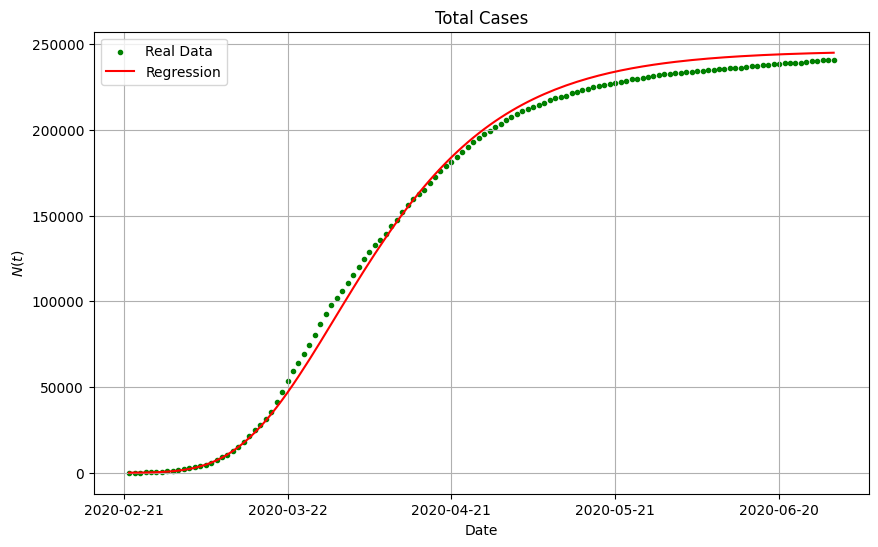
\includegraphics[width=0.6\linewidth]{plots/total_with_data}\\
        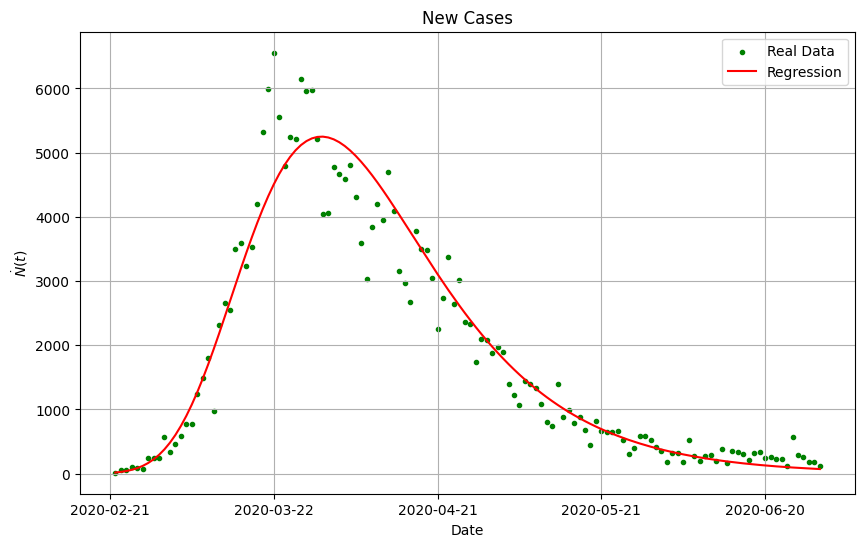
\includegraphics[width=0.6\linewidth]{plots/new_with_data}
        \caption{Comparison between the regressed equations and the real values}
        \label{fig:results}
    \end{figure}

\pagebreak

    \appendix
    \section{Data Sources}
    \begin{itemize}
        \item Covid infection data is available on the Covid section of the WHO website \url{https://data.who.int/dashboards/covid19/}
        \item Temperature data is available on the EU Copernicus Climate Data Store website \url{https://cds.climate.copernicus.eu/}
        \item Mobility data is available on the Google Covid19 Mobility Report website \url{https://www.google.com/covid19/mobility/}
    \end{itemize}
\end{document}